% lualatex presentation

\documentclass[svgnames]{beamer}
\usepackage[utf8]{inputenc}
\usepackage{fontspec}
\usepackage{arev}
\usepackage{beramono}
\usepackage{fontawesome}
\usepackage{listings}
\usepackage{hyperref}

\usetheme{default}
\setbeamertemplate{navigation symbols}
{%
%  \hspace{3em}
%  \vbox{%
%  \hbox{\insertslidenavigationsymbol}
%  \hbox{\insertframenavigationsymbol}
%  \hbox{\insertbackfindforwardnavigationsymbol}
%  \vspace{2em}}
}

\setbeamercolor{alerted text}{fg=red!70!black}
\setbeamercolor{structure}{fg=Navy}


\hypersetup{%
  pdftitle={Introduction to Version Control with Git}
  ,pdfauthor={Gert-Ludwig Ingold <gert.ingold@physik.uni-augsburg.de>}
  ,pdfsubject={Tutorial at EuroSciPy 2017, Erlangen 29.8.2017}
  ,pdfkeywords={Git, version control system, tutorial, EuroSciPy}
}

\lstset{%
  language=bash
  ,basicstyle={\ttfamily}
  ,escapechar=/
}

\graphicspath{{./images/}}

\begin{document}

\begin{frame}

 \vspace{1truecm}
 \begin{center}
  \structure{\large\textbf{Introduction to Version Control with Git}}\\[0.3truecm]
  \structure{Gert-Ludwig Ingold}

  \vspace{1.5truecm}
  \faicon{github}\ \ttfamily{\scriptsize https://github.com/gertingold/euroscipy-git-tutorial.git}
 \end{center}
\end{frame}

\begin{frame}
 \begin{center}
  \bfseries
  \uncover<1->{Do you write 100\% bugfree code with all features implemented from the very
	       beginning?}

  \vspace{0.2truecm}
  \uncover<2->{\textbullet}

  \vspace{0.2truecm}
  \uncover<2->{Do you collaborate with others?}

  \vspace{0.2truecm}
  \uncover<3->{\textbullet}

  \vspace{0.2truecm}
  \uncover<3->{Do you want to contribute to open software?}
 \end{center}
\end{frame}

\begin{frame}{A short history of version control}
 \begin{itemize}
  \item SCCS -- Source Code Control System (1972)
  \item RCS -- Revision Control System (1982)
  \item CVS -- Concurrent Versions System (1990)
  \item Subversion (2000)
  \item \alert{Git}, Mercurial, Bazaar (2005)
 \end{itemize}
\end{frame}

\begin{frame}{Centralized version control systems}
 \begin{center}
  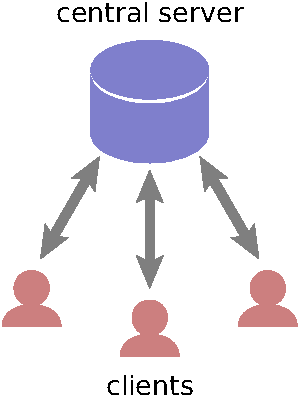
\includegraphics[width=\textwidth]{cvcs}
 \end{center}
\end{frame}

\end{document}
